\documentclass{beamer}
\usetheme{Darmstadt}

\usepackage[german]{babel}
\usepackage[utf8]{inputenc}

\title{Also sprach Zarathustra}
\subtitle{Ein Buch für Alle und Keinen}
\author{Richard Blažek, 4.A}
\date{}

\begin{document}
 \begin{frame}
\titlepage
\end{frame}

\begin{frame}
\frametitle{Friedrich Nietzsche}
\begin{minipage}{.49\textwidth}
\begin{itemize}
\item Deutscher Philosoph, 1844--1900
\item Sein Schnurrbart war gro\ss{}
\item Er hat das Opium benutzt
\item Zum Ende seines Lebens war er umnachtet
\end{itemize}
\end{minipage}
\begin{minipage}{.49\textwidth}
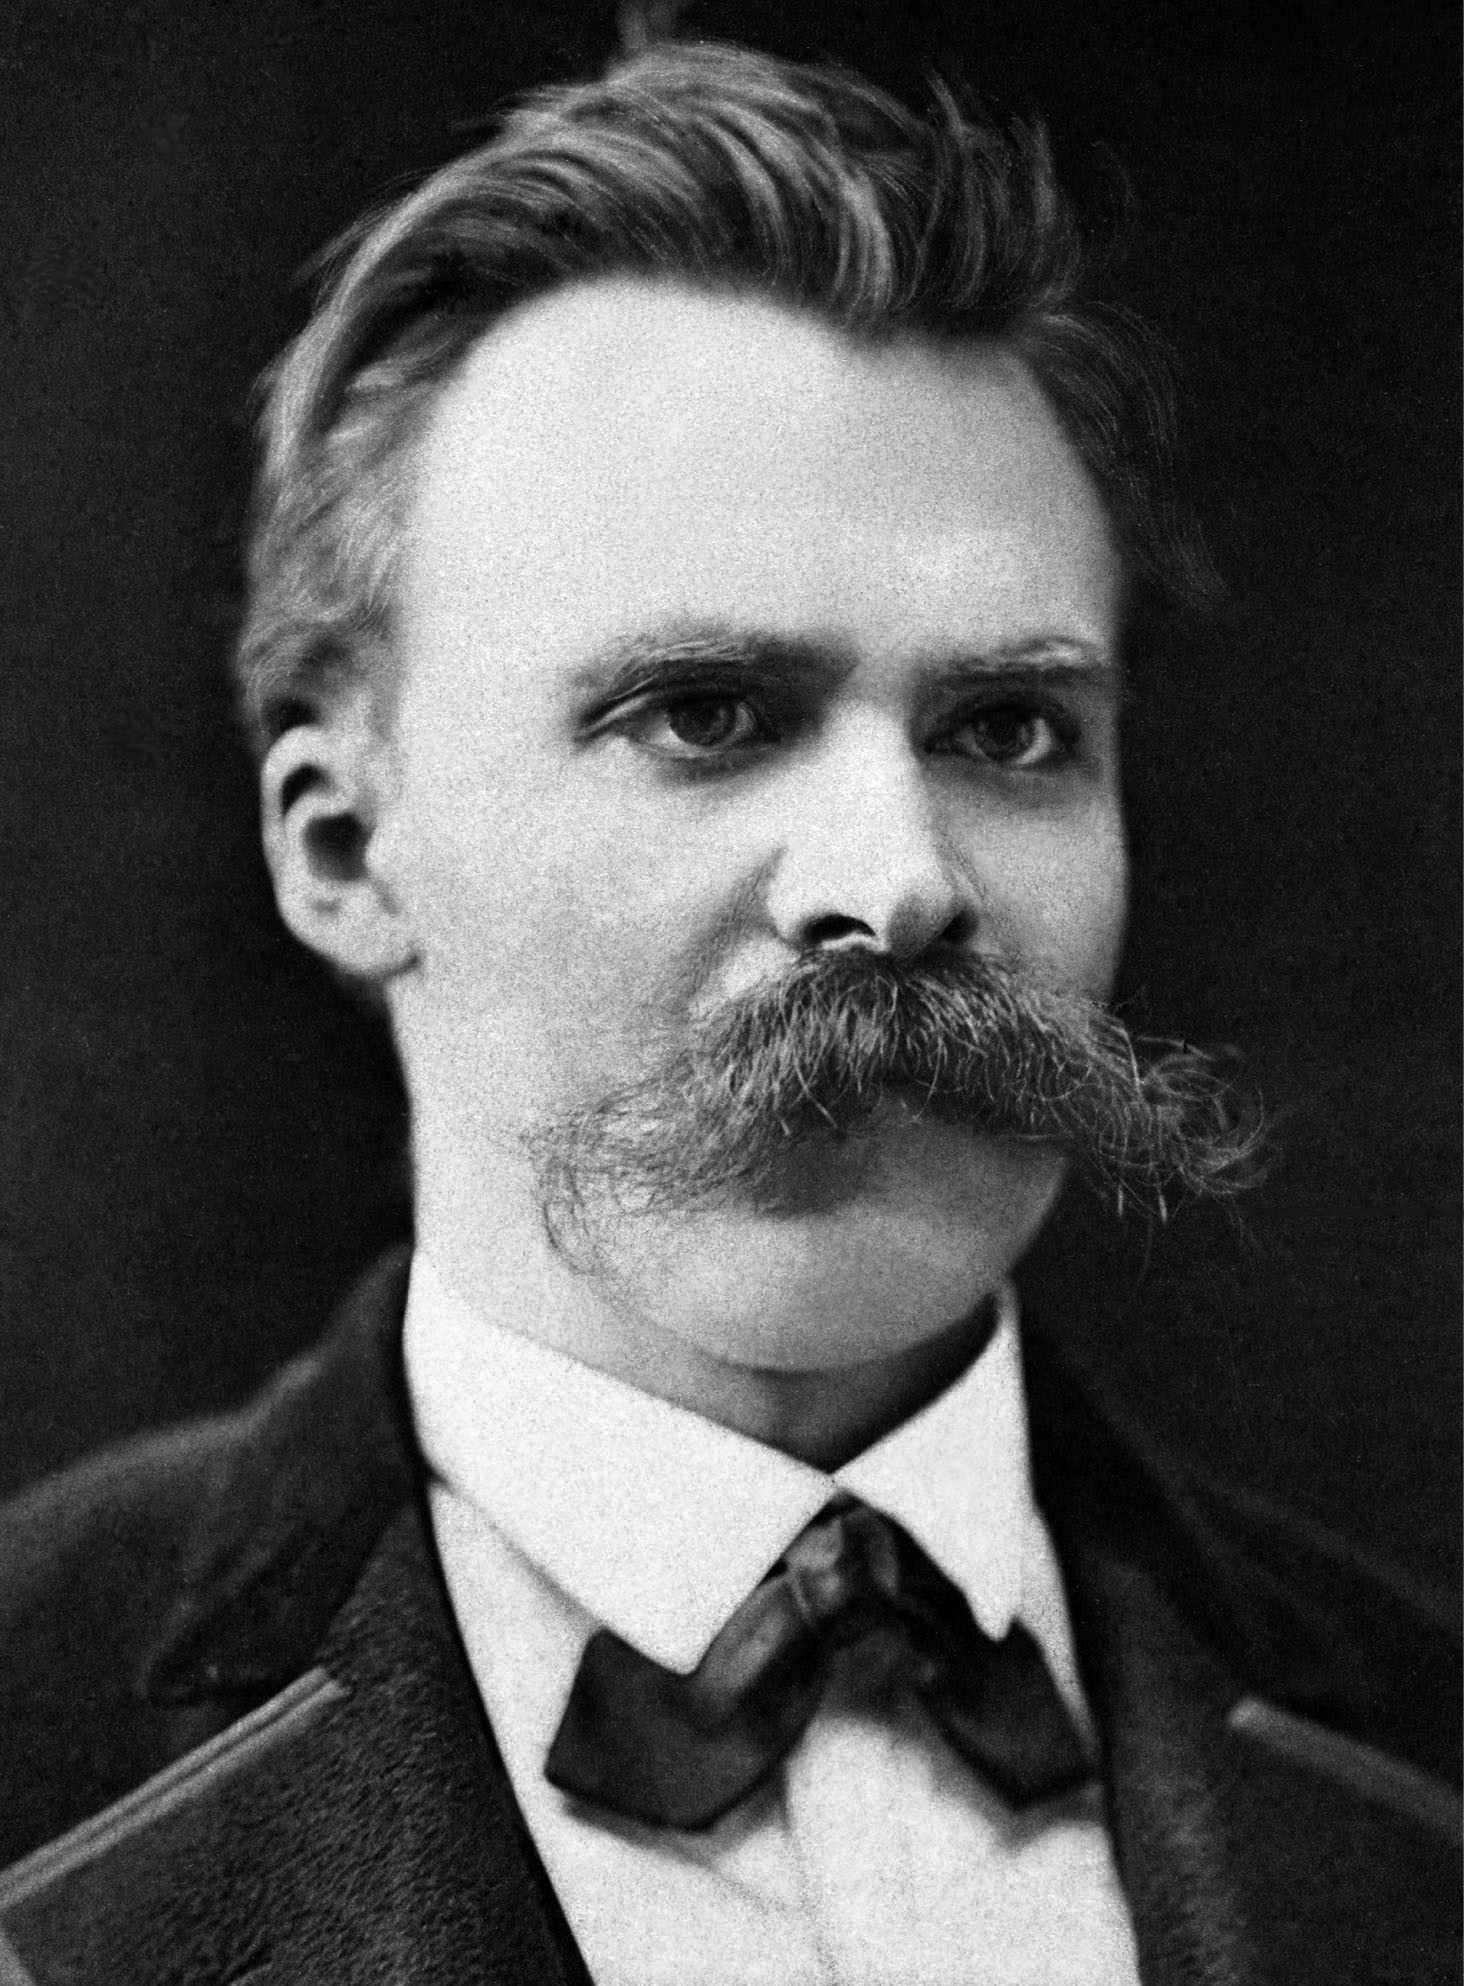
\includegraphics[width=\textwidth]{friedrich.jpg}
\end{minipage}
\end{frame}

\begin{frame}
\frametitle{Also sprach Zarathustra}
\begin{minipage}{.49\textwidth}
\begin{itemize}
\item Zarathustra war ein Eremit
\item Er wurde weise und wollte die Leute lehren
\item Er sagte, dass Gott tot ist
\end{itemize}
\end{minipage}
\begin{minipage}{.49\textwidth}

\includegraphics[width=\textwidth]{gottisttot.jpg}
\end{minipage}
\end{frame}

\begin{frame}
\frametitle{Der Übermensch}
\begin{minipage}{.49\textwidth}
\begin{itemize}
\item Zarathustra predigte über den Übermensch
\item Er warnte die Leute vor den letzten Mensch
\item Letzte Menschen werden einfache Leben wollen
\item Die Leute lachten über Zarathustra
\end{itemize}
\end{minipage}
\begin{minipage}{.49\textwidth}
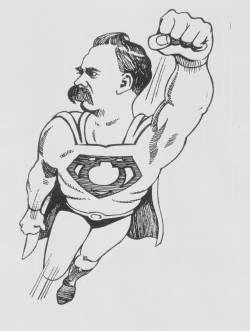
\includegraphics[width=\textwidth]{ubermensch.jpg}
\end{minipage}
\end{frame}

\begin{frame}
\frametitle{Die Reden Zarathustras}
\begin{minipage}{.49\textwidth}
\begin{itemize}
\item Zarathustra wanderte und predigte
\item Seine Anhänger wanderten mit ihm
\item Er sprach über verschiedene Dinge mit ihnen
\end{itemize}
\end{minipage}
\begin{minipage}{.49\textwidth}
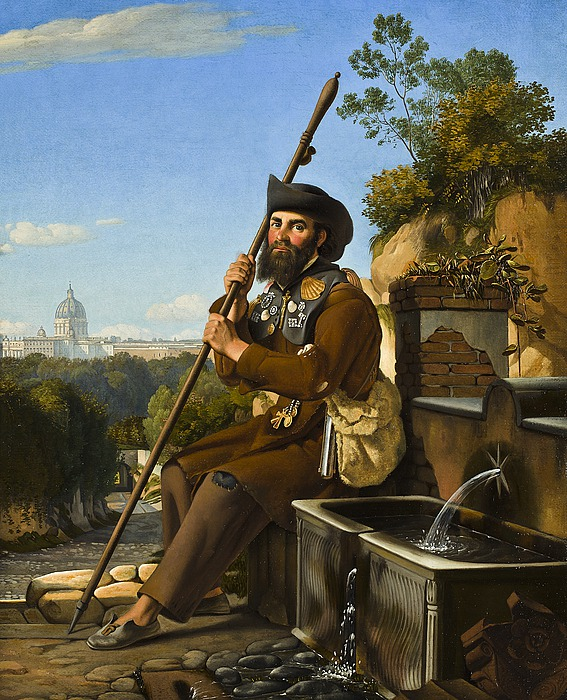
\includegraphics[width=\textwidth]{zarathustra.jpg}
\end{minipage}
\end{frame}

\begin{frame}
\frametitle{Andere Ideen}
\begin{minipage}{.49\textwidth}
\begin{itemize}
\item Ewige Wiederkunft: die Geschichte wiederholt sich -- immer
\item Wille zur Macht: vieldeutig, sich verbessern (die Fähigkeit) oder regieren (die Vorherrschaft)?
\end{itemize}
\end{minipage}
\begin{minipage}{.49\textwidth}

\includegraphics[width=\textwidth]{macht.jpg}
\end{minipage}
\end{frame}

\begin{frame}
\frametitle{Danke für euer Interesse}
\begin{center}

\includegraphics[height=0.8\textheight]{nietzscheisttot.jpg}
\end{center}
\end{frame}

\end{document}